\documentclass[conference]{IEEEtran}
\IEEEoverridecommandlockouts

\usepackage{cite}
\usepackage{amsmath,amssymb,amsfonts}
\usepackage{graphicx}
\usepackage{textcomp}
\usepackage{xcolor}
\usepackage{booktabs}
\usepackage{array}
\usepackage{url}
\usepackage{multirow}
\usepackage{float}
\usepackage{subcaption}

\begin{document}

\title{Adaptive Multi-Modal Fusion Transformer for Indian Sign Language Recognition}

\author{\IEEEauthorblockN{Tharunika S S}
\IEEEauthorblockA{\textit{Department of Computer Science and Engineering} \\
\textit{Sri Eshwar College of Engineering}\\
Coimbatore, Tamil Nadu, India \\
Email: tharunika.ss@sece.ac.in}
\and
\IEEEauthorblockN{L Rishi Raj}
\IEEEauthorblockA{\textit{Department of Computer Science and Engineering} \\
\textit{National Institute of Technology, Calicut}\\
Kozhikode, India \\
Email: rishi\_m240435cs@nitc.ac.in}
}

\maketitle

\begin{abstract}
Indian Sign Language (ISL) recognition is an important assistive vision task that aims to convert sign gestures into meaningful textual labels. The task is challenging because signs involve spatial hand-shape information, body posture, motion trajectory, and temporal gesture progression. This paper presents an Adaptive Multi-Modal Fusion Transformer framework for Indian Sign Language recognition using RGB video frames and pose landmarks. The proposed system contains two complementary branches. The RGB branch uses a ResNet50 backbone to extract frame-level visual features and a Transformer Encoder to model temporal dependencies across video frames. The pose branch uses MediaPipe Holistic landmarks to represent hand and body movement patterns. Multiple fusion strategies are evaluated, including RGB baseline, pose-only classification, late fusion, feature concatenation fusion, and adaptive fusion. Experiments are conducted on an eight-class subset of the INCLUDE dataset containing 103 videos. The RGB baseline and late fusion models achieve the highest test accuracy of 81.82\%, while the adaptive fusion model achieves 45.45\% and learns interpretable modality weights. The learned fusion weights assign 14.8\% importance to RGB and 85.2\% to pose, indicating that landmark trajectories contain meaningful gesture-related information. Grad-CAM and temporal attention analysis further show that the model focuses on hand-arm regions and middle frames corresponding to the gesture apex.
\end{abstract}

\begin{IEEEkeywords}
Indian Sign Language Recognition, Multi-Modal Fusion, ResNet50, Transformer Encoder, MediaPipe Holistic, Adaptive Fusion, Grad-CAM, Explainable AI
\end{IEEEkeywords}

\section{Introduction}

Sign language is a primary mode of communication for deaf and hard-of-hearing individuals. Indian Sign Language (ISL) is used by a large community in India, yet automatic ISL recognition remains less explored compared to American Sign Language and British Sign Language. A reliable ISL recognition system can support communication accessibility in education, healthcare, public services, and human-computer interaction.

Automatic sign language recognition is a difficult computer vision problem because a sign is not defined by a single image. Instead, it is formed by a sequence of hand movements, body posture changes, hand orientation, and facial or non-manual cues. Recognition systems must therefore understand both spatial information and temporal motion. RGB video frames provide rich appearance details such as hand shape, finger orientation, and body context. However, RGB-based methods are sensitive to illumination, background clutter, signer appearance, camera viewpoint, and clothing variations.

Pose-based representations provide another useful signal. By extracting body and hand landmarks, a model can focus on the geometric structure of the gesture rather than the full visual background. Pose landmarks are compact and often robust to appearance variations. However, pose extraction can be noisy when hands are blurred, occluded, or outside the frame. Pose-only systems may also lose fine-grained visual details such as hand shape and subtle finger orientation.

To address these limitations, this work proposes an Adaptive Multi-Modal Fusion Transformer for ISL recognition. The framework combines RGB video features and pose landmark sequences through a dual-branch architecture. The RGB branch uses ResNet50 and a Transformer Encoder, while the pose branch uses MediaPipe Holistic landmarks and temporal encoding. A learnable adaptive fusion module estimates modality weights for RGB and pose features before classification.

The main contributions of this work are:
\begin{enumerate}
    \item A dual-branch ISL recognition framework that processes RGB frames and pose landmarks.
    \item A ResNet50-Transformer RGB branch for spatial-temporal visual representation learning.
    \item A MediaPipe-based pose branch for hand and body landmark trajectory modelling.
    \item A Softmax-gated adaptive fusion module that learns modality weights for RGB and pose features.
    \item An ablation and explainability study comparing five model configurations using accuracy, F1-score, confusion analysis, Grad-CAM, and temporal attention maps.
\end{enumerate}

The remainder of this paper is organized as follows. Section II reviews related work. Section III presents the system architecture. Section IV describes the methodology and dataset. Section V reports experimental results and analysis. Section VI concludes the study and outlines future directions.

\section{Related Work}

Recent progress in deep learning has significantly improved sign language recognition systems. Early methods used hand-crafted descriptors such as Histogram of Oriented Gradients, Scale-Invariant Feature Transform, optical flow, and skin-color segmentation, followed by classifiers such as Support Vector Machines or Hidden Markov Models. Although these methods were computationally efficient, they were sensitive to background variations and required careful feature engineering.

\subsection{RGB-Based Sign Recognition}

RGB-based sign recognition methods use raw video frames as input. Convolutional Neural Networks (CNNs) are commonly used to extract spatial representations from individual frames. To model temporal gesture information, CNNs are often combined with recurrent networks such as LSTM or GRU models. More recently, Transformer-based temporal encoders have been used for video understanding because self-attention can capture relationships between frames without sequential recurrence.

Pretrained CNN backbones such as ResNet50 provide strong frame-level feature extraction. In sign recognition, these features can capture hand shape, body position, and contextual appearance information. However, RGB-only approaches can be affected by lighting variations, camera background, signer clothing, and other visual noise.

\subsection{Pose and Landmark-Based Recognition}

Pose-based recognition methods use body and hand keypoints rather than full image pixels. Landmark extraction tools such as OpenPose and MediaPipe Holistic make it possible to represent a gesture as a sequence of coordinate vectors. This representation reduces background dependency and provides direct access to hand and body motion trajectories.

Despite these advantages, landmark-based methods have limitations. Hand landmarks may be incorrectly detected during fast motion, self-occlusion, or low-resolution frames. In such cases, important information may be missing from the coordinate representation. Therefore, pose information alone may not be sufficient for robust sign recognition.

\subsection{Multi-Modal Fusion}

Multi-modal fusion combines complementary signals from multiple input sources. In sign language recognition, RGB frames and pose landmarks provide different but related information. RGB captures appearance and hand shape, while pose captures movement geometry. Fusion methods can be broadly categorized as early fusion, late fusion, feature concatenation, and adaptive fusion.

Late fusion combines predictions from separate models and is simple to implement. Feature concatenation combines intermediate embeddings before classification. Adaptive fusion learns how much importance should be assigned to each modality. This work evaluates these fusion strategies and analyzes whether learned modality weighting improves ISL recognition on a small INCLUDE dataset subset.

\section{System Architecture}

The proposed framework consists of five major components: input video sampling, RGB feature extraction, pose landmark extraction, temporal modelling, and multimodal fusion. The overall objective is to classify each video into one of the predefined ISL sign classes.

\subsection{Input Processing}

Each input video is uniformly sampled into 16 frames. Uniform sampling ensures that the model observes the beginning, middle, and end of the sign gesture. Each RGB frame is resized to $224 \times 224$ pixels and normalized using ImageNet statistics. In parallel, MediaPipe Holistic is used to extract pose and hand landmark coordinates from the corresponding frames.

\subsection{RGB Branch}

The RGB branch processes visual appearance information. A pretrained ResNet50 model is used as the frame-level feature extractor. The final classification layer is removed, and the backbone produces a 2048-dimensional feature vector for each sampled frame. These features are projected to a 512-dimensional space and passed to a Transformer Encoder for temporal modelling.

Let the sampled RGB sequence be represented as:
\begin{equation}
X_{rgb} = \{x_1, x_2, ..., x_T\}
\end{equation}
where $T=16$. The ResNet50 backbone extracts frame-level features:
\begin{equation}
f_t = ResNet50(x_t), \quad f_t \in \mathbb{R}^{2048}
\end{equation}
The sequence is projected and processed by the Transformer Encoder:
\begin{equation}
z_{rgb} = Transformer(W_{rgb}F_{rgb} + P_{rgb})
\end{equation}
where $P_{rgb}$ denotes learnable positional embeddings. Temporal average pooling is applied to obtain the final RGB embedding.

\subsection{Pose Branch}

The pose branch captures geometric hand and body motion using MediaPipe Holistic landmarks. For each sampled frame, the system extracts 33 body pose landmarks, 21 left-hand landmarks, and 21 right-hand landmarks. Pose landmarks contain $(x,y,z,\text{visibility})$ values, while hand landmarks contain $(x,y,z)$ values. After concatenation, each frame is represented as a 258-dimensional coordinate vector.

The pose sequence is represented as:
\begin{equation}
P = \{p_1, p_2, ..., p_T\}
\end{equation}
where each $p_t \in \mathbb{R}^{258}$ contains landmark coordinates for the corresponding frame. The coordinate features are projected to a 256-dimensional embedding space, combined with learnable temporal positional embeddings, and processed using a 4-layer Transformer Encoder with 4 attention heads:
\begin{equation}
z_{pose} = Transformer(W_{pose}P + P_{pose})
\end{equation}
The pooled pose representation is then projected to 512 dimensions so that it can be aligned and fused with the RGB representation.

\subsection{Adaptive Fusion Module}

The adaptive fusion module combines RGB and pose embeddings using learnable modality weights. The RGB and pose embeddings are concatenated and passed through a small gating network:
\begin{equation}
[\alpha,\beta] = Softmax(MLP([z_{rgb};z_{pose}]))
\end{equation}
where $\alpha$ represents the RGB weight and $\beta$ represents the pose weight. The Softmax operation ensures:
\begin{equation}
\alpha + \beta = 1
\end{equation}

The final fused representation is computed as:
\begin{equation}
z_{fused} = \alpha z_{rgb} + \beta z_{pose}
\end{equation}
The fused feature vector is then passed to a fully connected classifier to predict the sign class.

\begin{figure}[htbp]
\centering
\fbox{\begin{minipage}{0.46\textwidth}
\centering
\textbf{Input ISL Video}\\
$\downarrow$\\
Uniform Sampling: 16 Frames\\
$\downarrow$\\
\begin{tabular}{c c}
RGB Frames & Pose Landmarks\\
$\downarrow$ & $\downarrow$\\
ResNet50 + Transformer & MediaPipe + Transformer\\
$\downarrow$ & $\downarrow$\\
$z_{rgb}$ & $z_{pose}$\\
\end{tabular}\\
$\downarrow$\\
Adaptive Fusion $(\alpha,\beta)$\\
$\downarrow$\\
Classifier\\
$\downarrow$\\
Predicted Sign
\end{minipage}}
\caption{Proposed Adaptive Multi-Modal Fusion Transformer architecture for Indian Sign Language recognition.}
\label{fig:architecture}
\end{figure}

\section{Methodology}

The methodology follows a modular pipeline consisting of dataset preparation, preprocessing, model training, fusion evaluation, and explainability analysis. The implementation was performed using Python and PyTorch. OpenCV was used for video processing, MediaPipe Holistic was used for landmark extraction, and scikit-learn was used for evaluation metrics.

\subsection{Dataset Description}

Experiments were conducted on an eight-class subset of the INCLUDE Indian Sign Language dataset containing 103 videos. The selected adjective classes were loud (21 videos), quiet (21 videos), happy (21 videos), sad (8 videos), Beautiful (8 videos), Ugly (8 videos), Deaf (8 videos), and Blind (8 videos). The dataset was divided into 82 training samples, 10 validation samples, and 11 testing samples. This subset was selected to evaluate the behaviour of RGB appearance features, pose landmark features, and different fusion strategies under a small-data experimental setting.

\begin{table}[htbp]
\centering
\caption{Dataset Split Summary}
\begin{tabular}{lc}
\toprule
Split & Number of Videos \\
\midrule
Training & 82 \\
Validation & 10 \\
Testing & 11 \\
\bottomrule
\end{tabular}
\label{tab:split}
\end{table}

\begin{table}[htbp]
\centering
\caption{Selected ISL Classes}
\begin{tabular}{lc}
\toprule
Class ID & Class Label \\
\midrule
1 & loud \\
2 & quiet \\
3 & happy \\
4 & sad \\
5 & Beautiful \\
6 & Ugly \\
7 & Deaf \\
8 & Blind \\
\bottomrule
\end{tabular}
\label{tab:classes}
\end{table}



\begin{figure}[H]
\centering
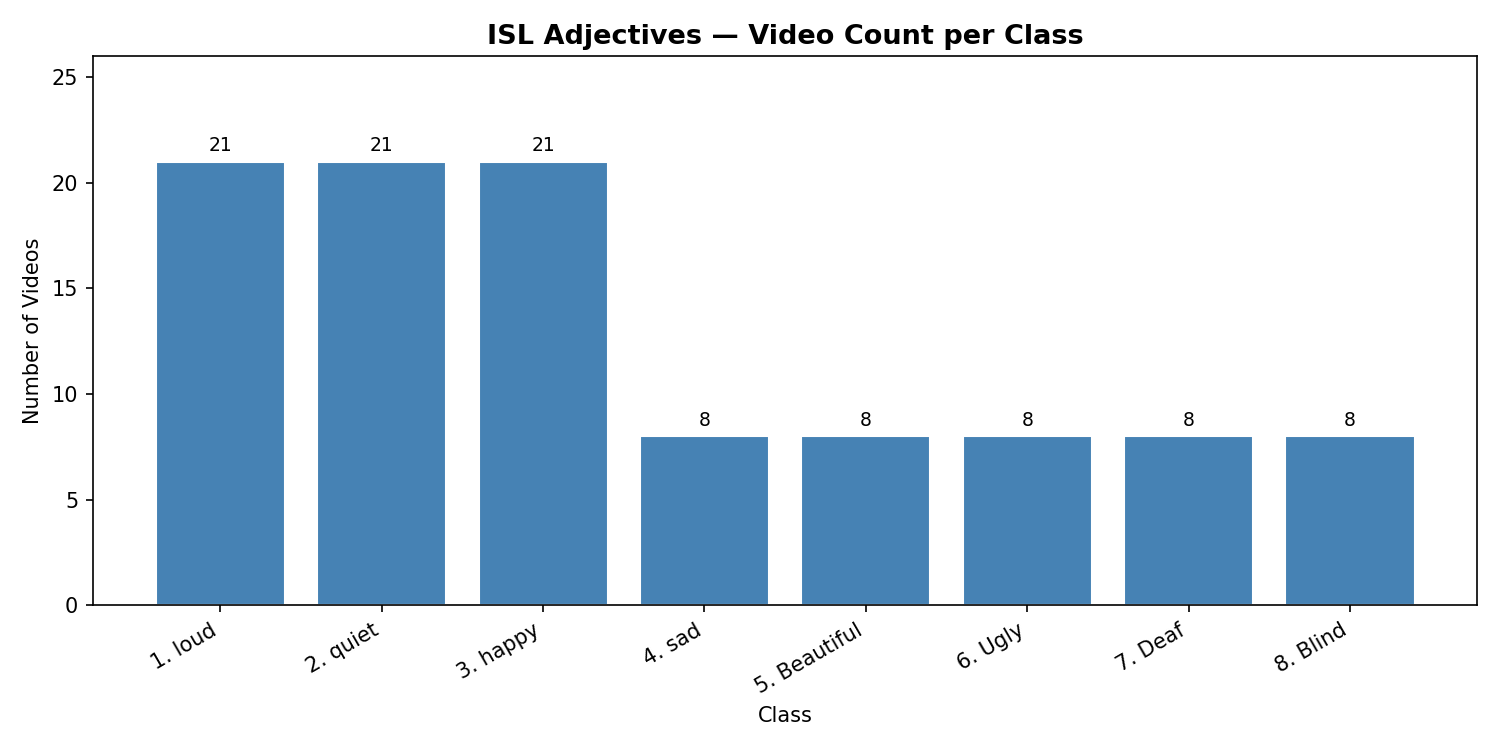
\includegraphics[width=0.95\linewidth]{results/5b3aae8d-234d-4954-9e4c-91688e5b0f6d.png}
\caption{Video count distribution across the selected ISL adjective classes.}
\label{fig:class_distribution}
\end{figure}

\subsection{Preprocessing}

Each video is uniformly sampled into 16 frames. RGB frames are resized to $224 \times 224$ pixels and normalized before being passed to the ResNet50 backbone. Pose landmarks are extracted using MediaPipe Holistic and saved as temporal coordinate sequences. This avoids running landmark extraction during training and improves reproducibility.

\subsection{Training Configuration}

The models were trained using CrossEntropyLoss and the Adam optimizer with a learning rate of $1 \times 10^{-4}$. The experiments were conducted for 10 epochs due to the small dataset size. Evaluation was performed using test accuracy, precision, recall, Macro F1-score, and parameter count.

\begin{table}[htbp]
\centering
\caption{Training Configuration}
\begin{tabular}{lc}
\toprule
Parameter & Value \\
\midrule
Frames per video & 16 \\
Image size & $224 \times 224$ \\
Backbone & ResNet50 \\
Optimizer & Adam \\
Learning rate & $1 \times 10^{-4}$ \\
Epochs & 10 \\
Number of classes & 8 \\
\bottomrule
\end{tabular}
\label{tab:config}
\end{table}

\begin{figure*}[t]
\centering
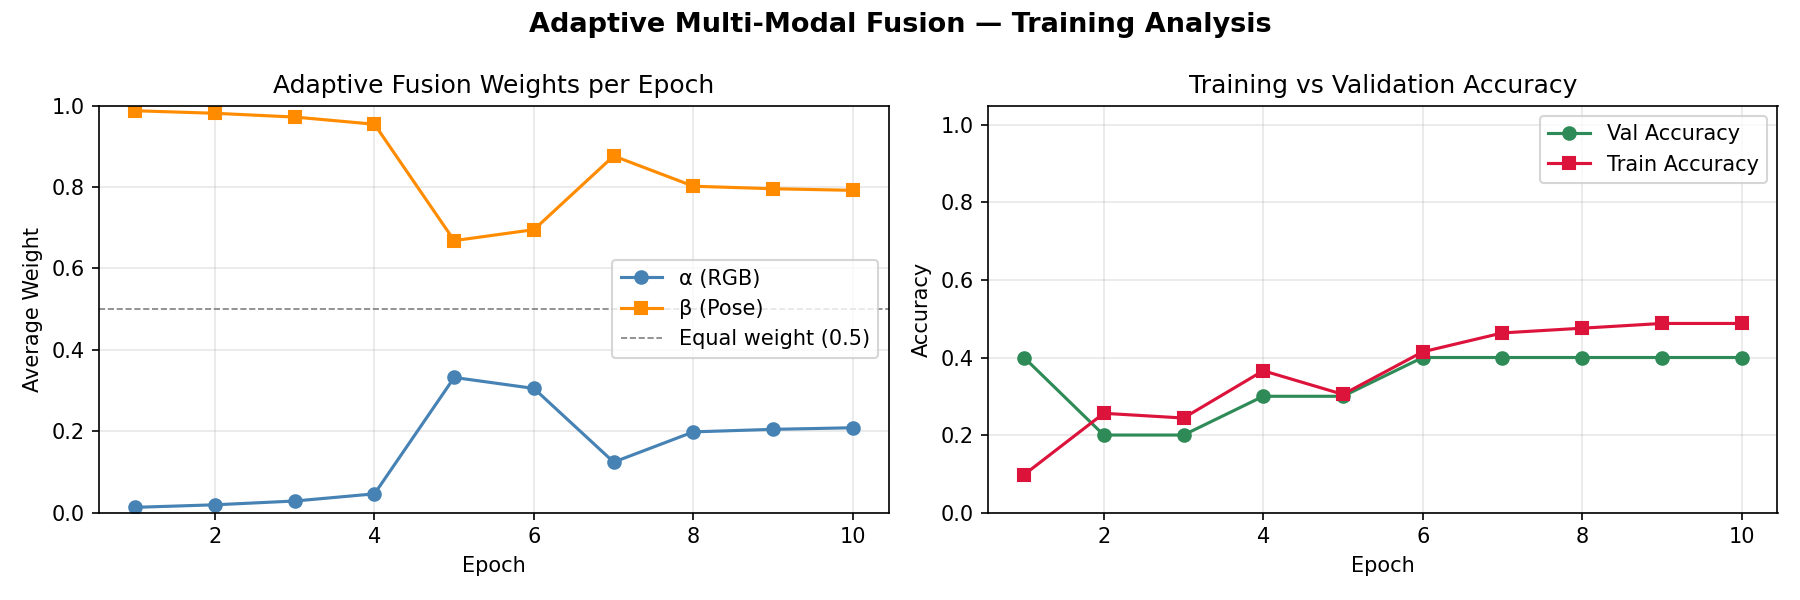
\includegraphics[width=\textwidth]{results/91598b88-fb0b-4fad-93d8-b7dd5ecde646.png}
\caption{Adaptive multi-modal fusion training analysis. The left plot shows the learned RGB and pose fusion weights across epochs, while the right plot compares training and validation accuracy.}
\label{fig:training_analysis}
\end{figure*}

\section{Evaluation and Results}

Ablation experiments were performed to evaluate the contribution of each component. Five models were compared: RGB baseline, pose-only model, late fusion, feature concatenation fusion, and adaptive fusion.

\begin{table*}[htbp]
\centering
\caption{Performance Comparison of Evaluated Models}
\resizebox{\textwidth}{!}{%
\begin{tabular}{lccccccc}
\toprule
Model Configuration & Train Acc (\%) & Val Acc (\%) & Test Acc (\%) & Precision & Recall & Macro F1 & Parameter Count \\
\midrule
RGB Baseline & 91.46 & 90.00 & \textbf{81.82} & 0.5000 & 0.5000 & 0.5000 & 37,178,952 \\
Pose Only & 32.93 & 60.00 & 9.09 & 0.0312 & 0.1250 & 0.0500 & 5,332,744 \\
Late Fusion & 76.83 & 70.00 & \textbf{81.82} & \textbf{0.5417} & \textbf{0.5625} & \textbf{0.5208} & 42,511,696 \\
Feature Concat Fusion & 59.76 & 60.00 & 54.55 & 0.2812 & 0.3750 & 0.3000 & 42,704,456 \\
Adaptive Fusion & 40.24 & 40.00 & 45.45 & 0.1027 & 0.2500 & 0.1409 & 19,264,650 \\
\bottomrule
\end{tabular}%
}
\label{tab:results}
\end{table*}

\begin{figure}[H]
\centering
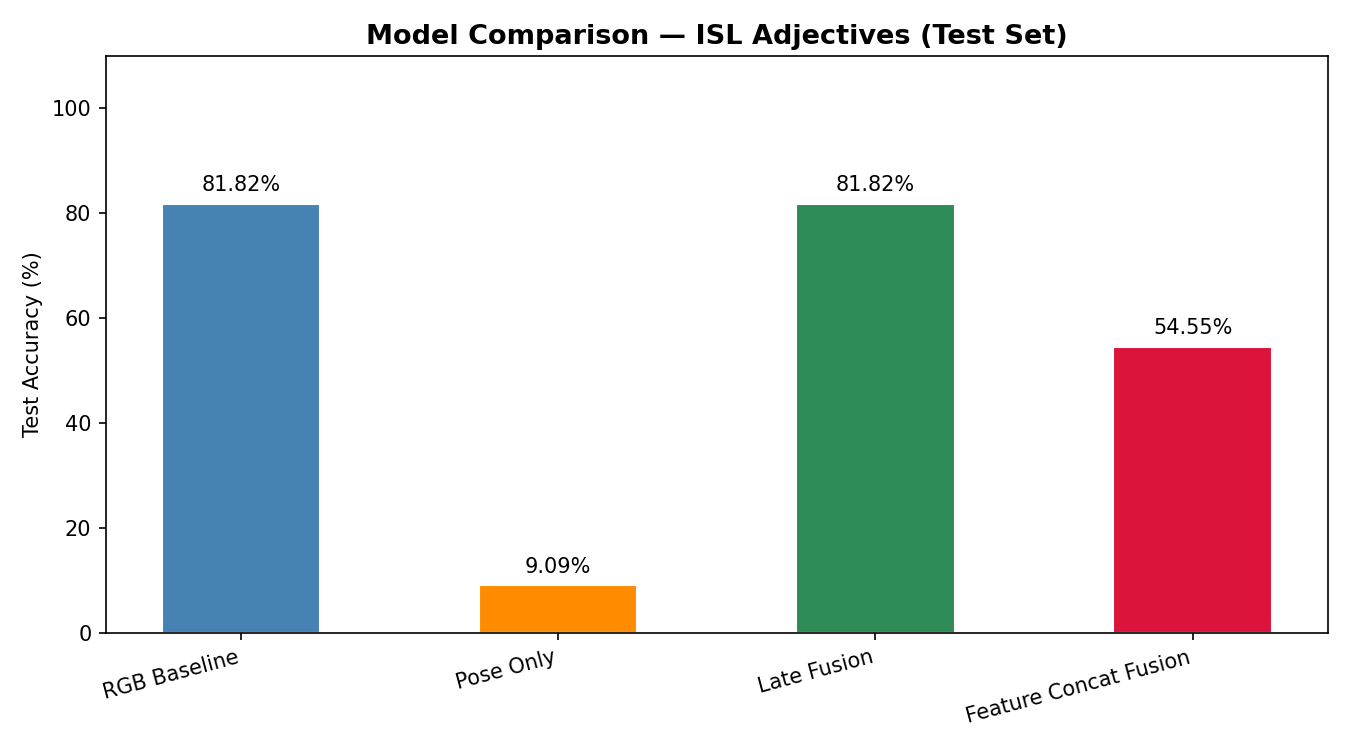
\includegraphics[width=0.95\linewidth]{results/756afa72-7d1e-4490-867c-2bc6034ef311.png}
\caption{Test accuracy comparison of RGB baseline, pose-only, late fusion, and feature concatenation fusion models on the ISL adjectives test set.}
\label{fig:model_comparison}
\end{figure}

\subsection{Performance Analysis}

The RGB baseline and late fusion models achieved the highest test accuracy of 81.82\%. This shows that RGB visual appearance features are highly effective for the selected ISL subset. Late fusion also achieved the highest Macro F1-score of 0.5208, indicating that pose information provides complementary benefit when combined at the prediction level.

The pose-only model achieved only 9.09\% test accuracy. This weak performance is mainly due to landmark tracking noise, coordinate-level self-occlusion, and the loss of fine-grained hand-shape information. Although pose coordinates are compact and lighting-invariant, they were not strong enough as a standalone modality for this small dataset.

Feature concatenation fusion and adaptive fusion performed lower than the RGB baseline. These methods increase learnable model capacity and require stronger joint optimization of multimodal feature spaces. With only 82 training samples, the feature-level fusion models showed signs of overfitting. The adaptive fusion model, however, remains useful because it provides interpretable modality weights and reveals how the model balances RGB and pose signals.

\subsection{Fusion Weight Analysis}

The adaptive fusion model learned average modality weights of 14.8\% for RGB and 85.2\% for pose. This indicates that the model assigned greater importance to pose landmark trajectories.

\begin{table}[htbp]
\centering
\caption{Average Adaptive Fusion Weights}
\begin{tabular}{lc}
\toprule
Modality & Average Weight \\
\midrule
RGB $(\alpha)$ & 14.8\% \\
Pose $(\beta)$ & 85.2\% \\
\bottomrule
\end{tabular}
\label{tab:weights}
\end{table}

Although the adaptive gate strongly preferred pose features, the pose-only classifier performed poorly. This explains why adaptive fusion did not outperform the RGB baseline. The gate identified pose as a cleaner and illumination-invariant cue, but the underperforming pose branch reduced the final fused accuracy. This result suggests that pose trajectories contain useful gesture information, but the pose encoder requires stronger preprocessing, more samples, and better regularization.

\subsection{Confusion Analysis}

The confusion matrix of the evaluated test set is shown in Fig.~\ref{fig:confusion_matrix}. The confusion analysis showed that several visually similar signs were misclassified. The most common error was loud classified as happy, because both gestures involve raising open hands near the ears. Another frequent error was quiet classified as Blind, because both signs involve hand movements near facial regions such as the lips or eyes.


\begin{figure}[H]
\centering
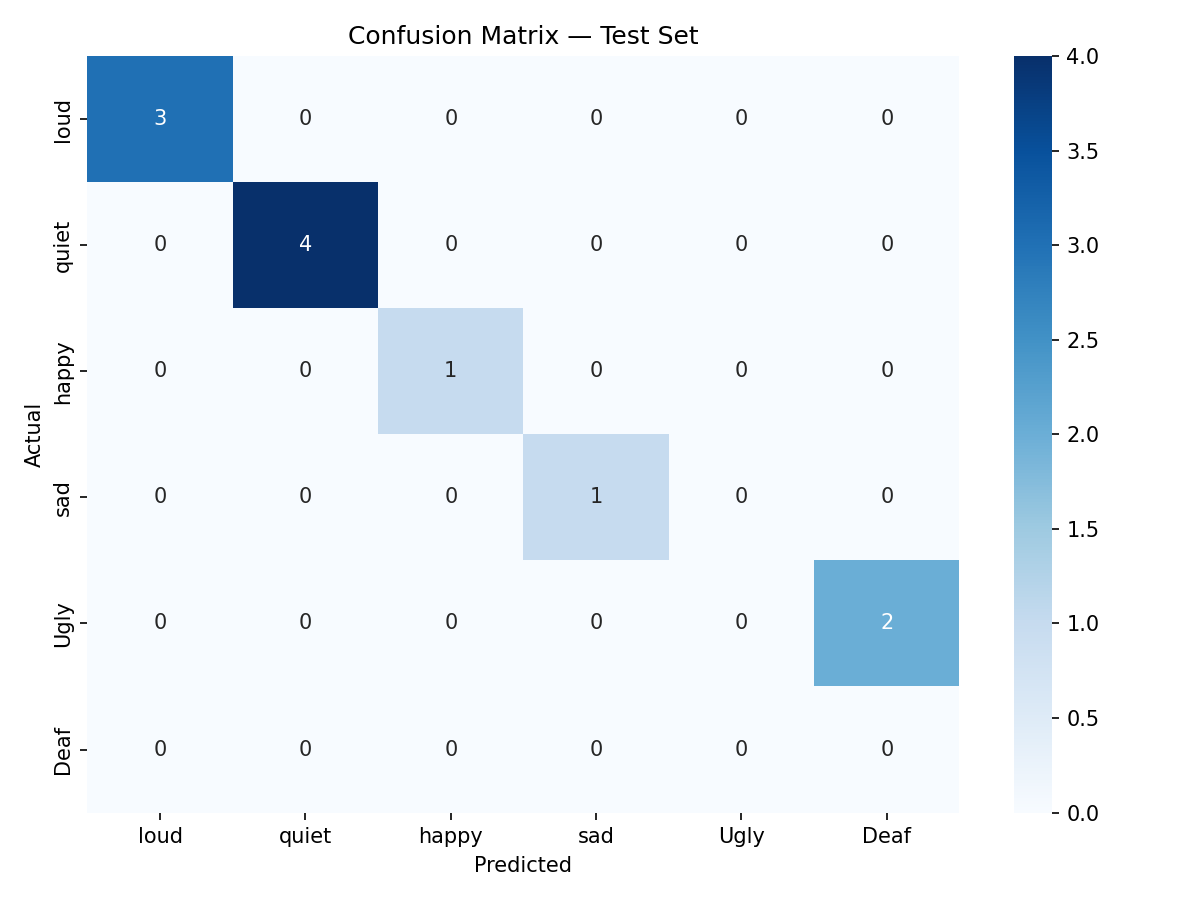
\includegraphics[width=0.95\linewidth]{results/5d897fef-a628-4a86-a7c5-630ae5559014.png}
\caption{Confusion matrix of the proposed adaptive fusion model on the test set.}
\label{fig:confusion_matrix}
\end{figure}

\begin{table}[htbp]
\centering
\caption{Commonly Confused Class Pairs}
\begin{tabular}{lc}
\toprule
Confused Pair & Error Count \\
\midrule
loud $\rightarrow$ happy & 42 \\
quiet $\rightarrow$ Blind & 21 \\
Deaf $\rightarrow$ Blind & 9 \\
sad $\rightarrow$ Blind & 8 \\
Beautiful $\rightarrow$ Blind & 8 \\
\bottomrule
\end{tabular}
\label{tab:confusion}
\end{table}

\begin{figure*}[t]
\centering
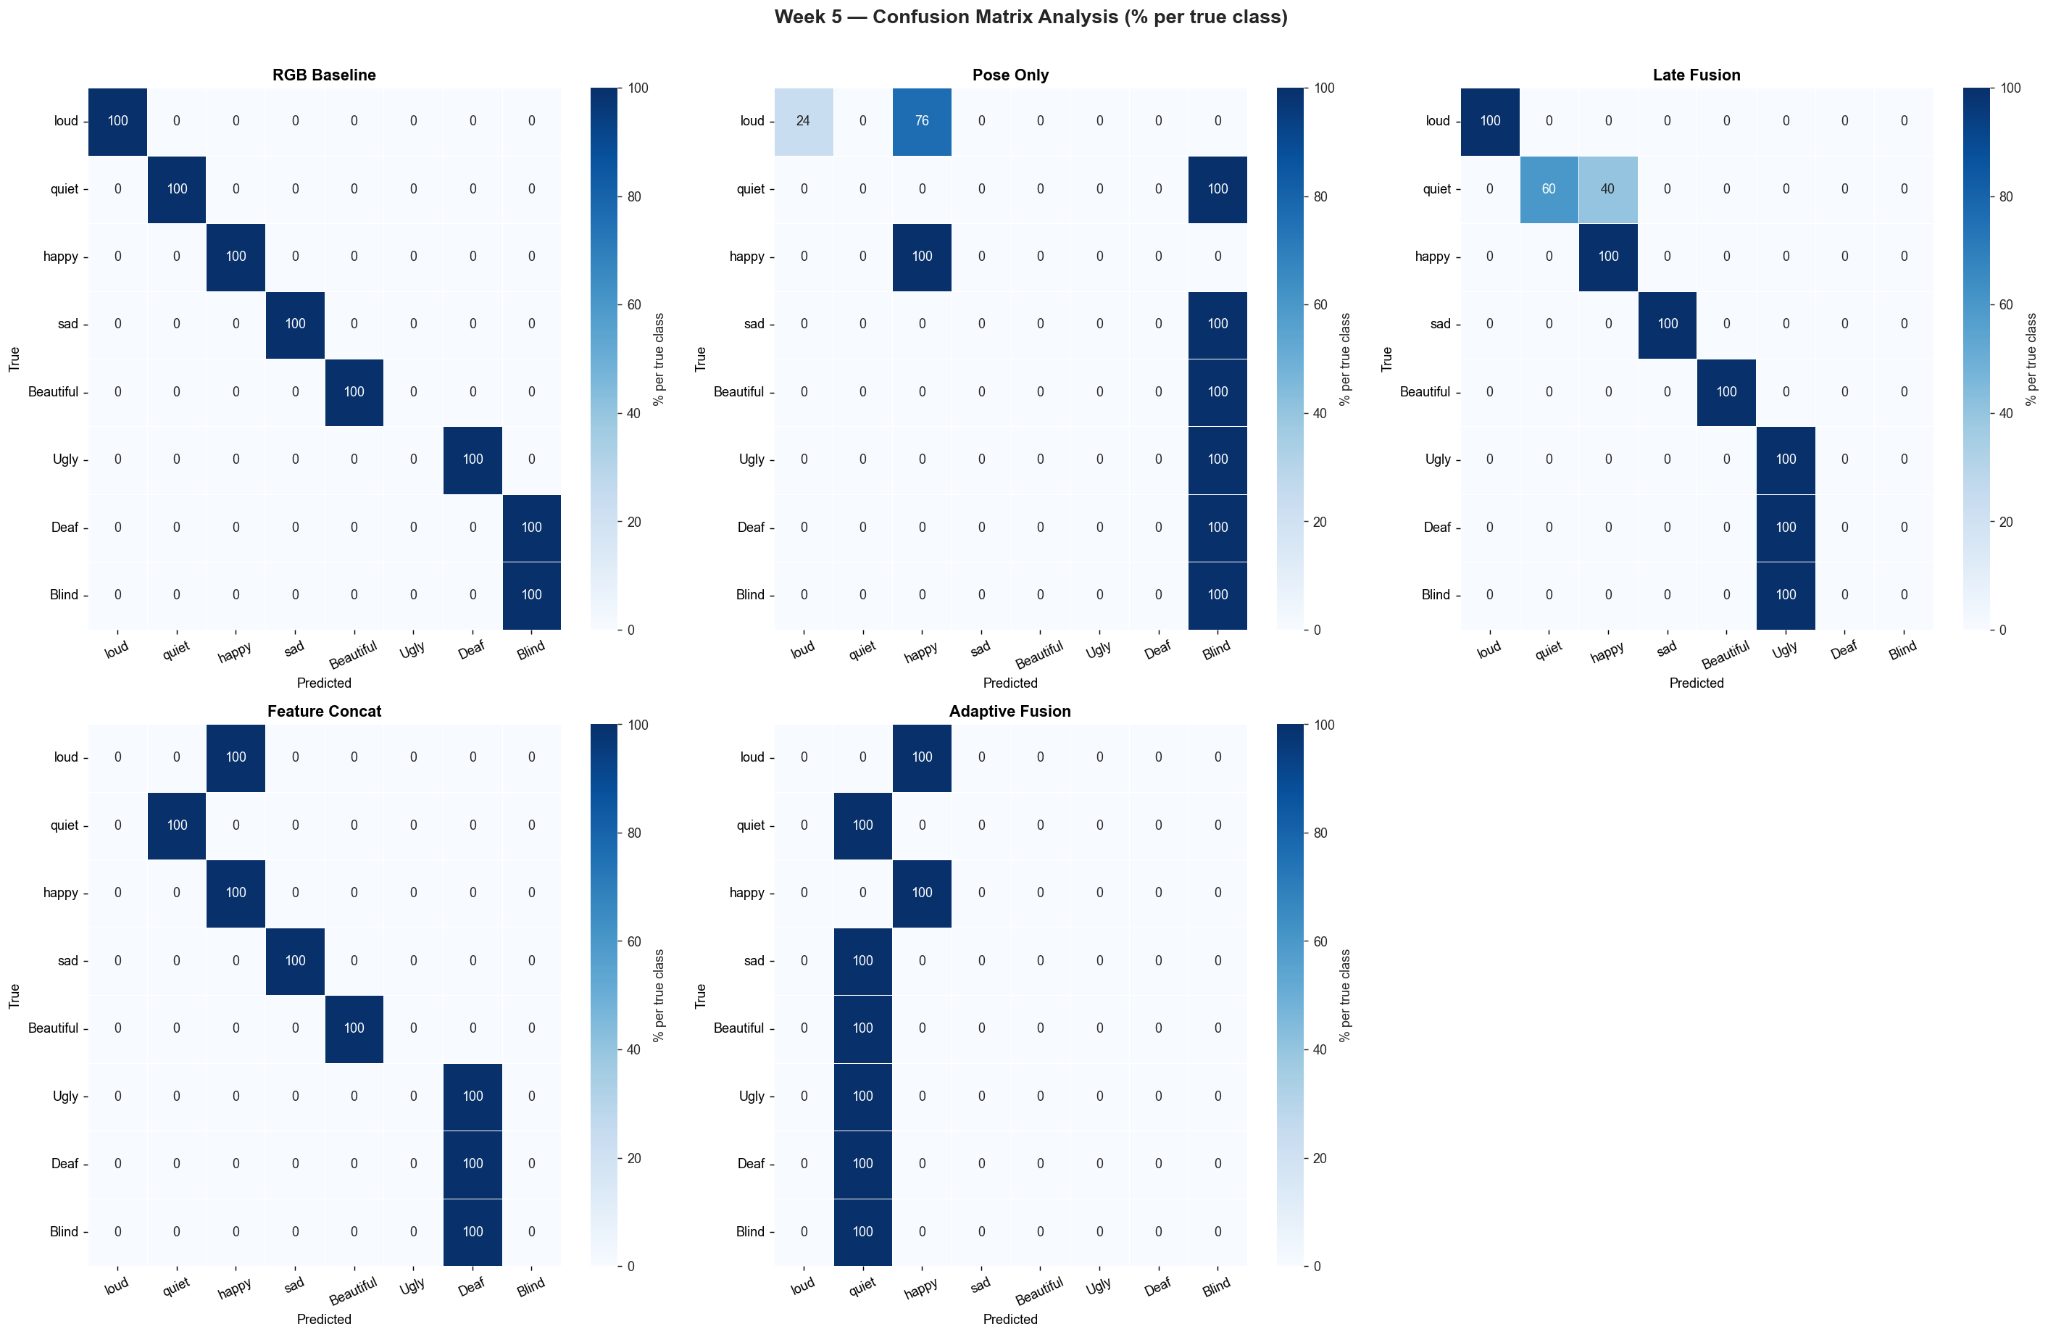
\includegraphics[width=\textwidth]{results/035f0868-2e6a-4342-acad-ae0177369eea.png}
\caption{Per-class confusion matrix comparison for RGB baseline, pose-only, late fusion, feature concatenation, and adaptive fusion models.}
\label{fig:week5_confusion}
\end{figure*}

\subsection{Explainability Analysis}

Grad-CAM visualization was used to analyze the spatial focus of the RGB branch. Correct predictions showed activation around the hands, arms, and face regions. This indicates that the model focuses on meaningful gesture areas rather than only background information.

Temporal attention maps were used to analyze the Transformer Encoder. The attention weights were strongest around frames 6--12. These middle frames correspond to the semantic apex of the gesture, while the beginning and ending frames mostly contain transition movement. This shows that the Transformer learns useful temporal importance patterns, as shown in Fig.~\ref{fig:attention_quiet1}, Fig.~\ref{fig:attention_quiet2}, Fig.~\ref{fig:attention_sad}, and Fig.~\ref{fig:attention_loud}.

\begin{figure*}[t]
\centering
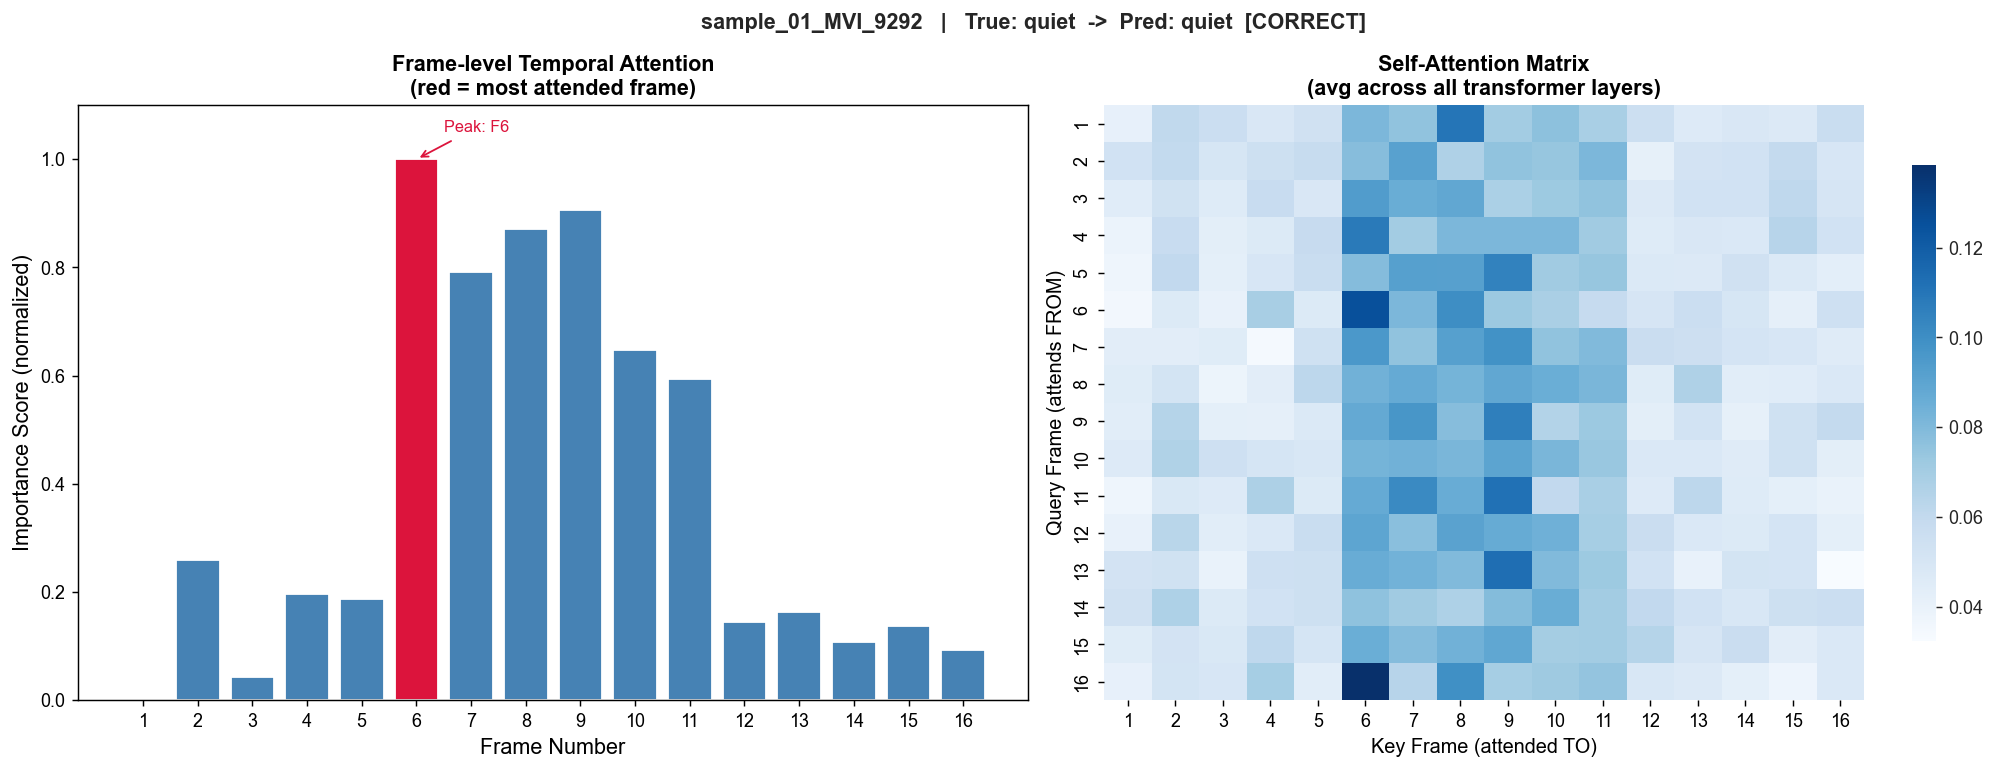
\includegraphics[width=\textwidth]{results/4a09f266-8237-481c-b4ab-80f2f25bc3bd.png}
\caption{Temporal attention visualization for a correctly classified quiet sample. The highlighted frame indicates the most attended temporal region.}
\label{fig:attention_quiet1}
\end{figure*}

\begin{figure*}[t]
\centering
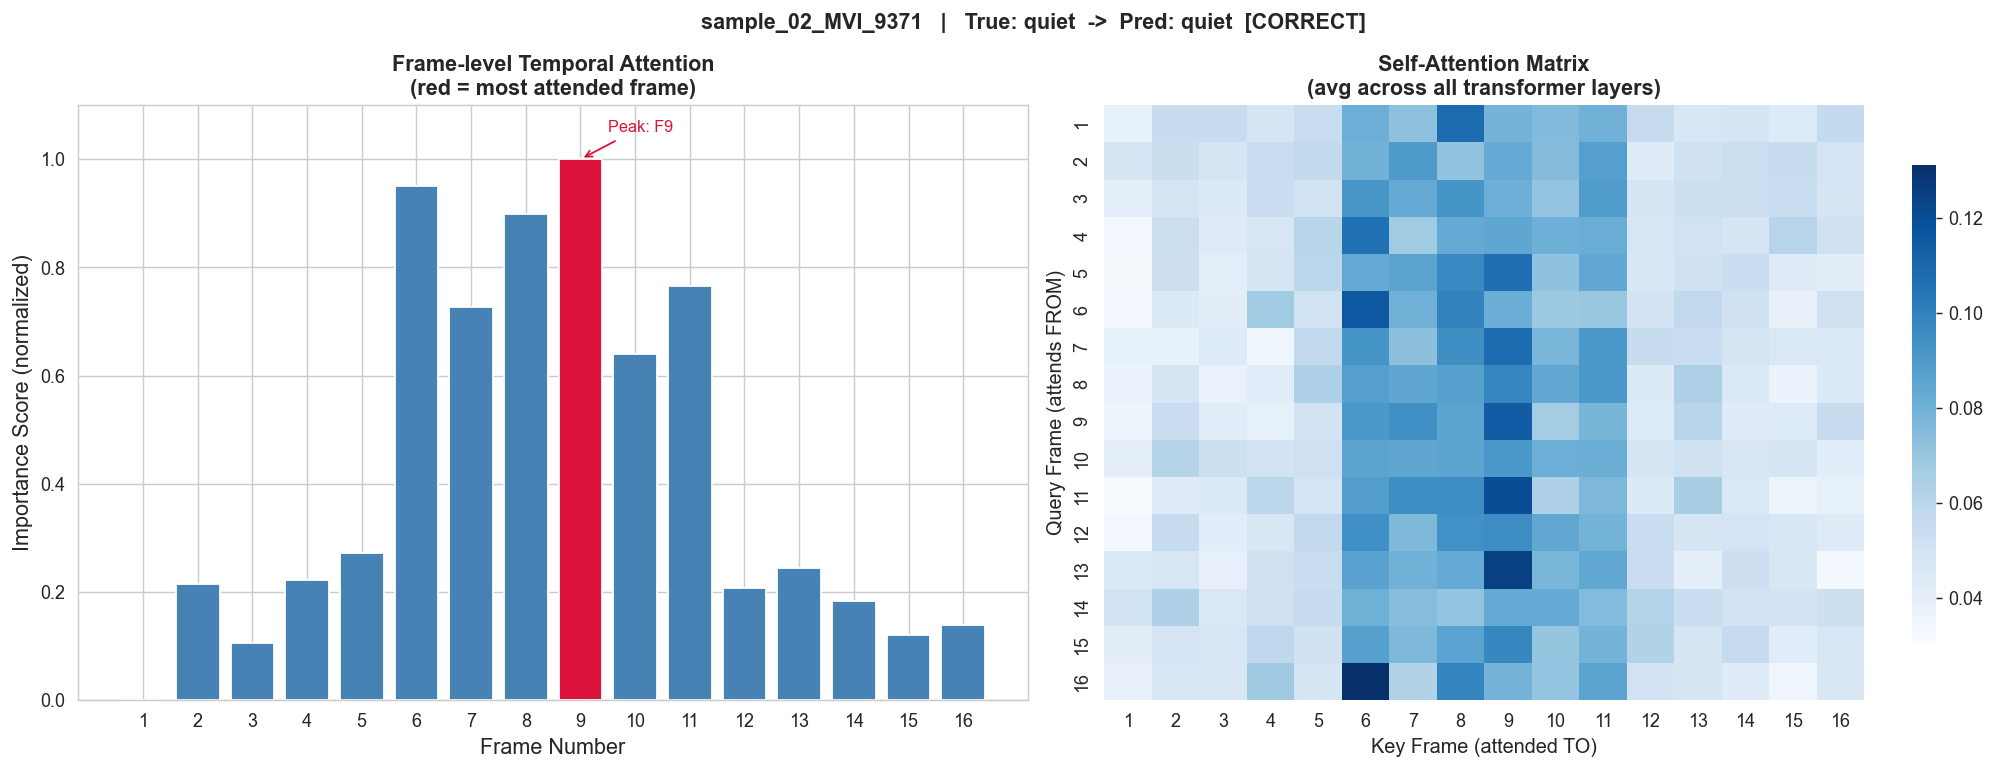
\includegraphics[width=\textwidth]{results/6268fd97-b6a1-4d25-8621-0ed0b064563e.png}
\caption{Temporal attention visualization for a correctly classified quiet sample with the highest attention on frame 9.}
\label{fig:attention_quiet2}
\end{figure*}

\begin{figure*}[t]
\centering
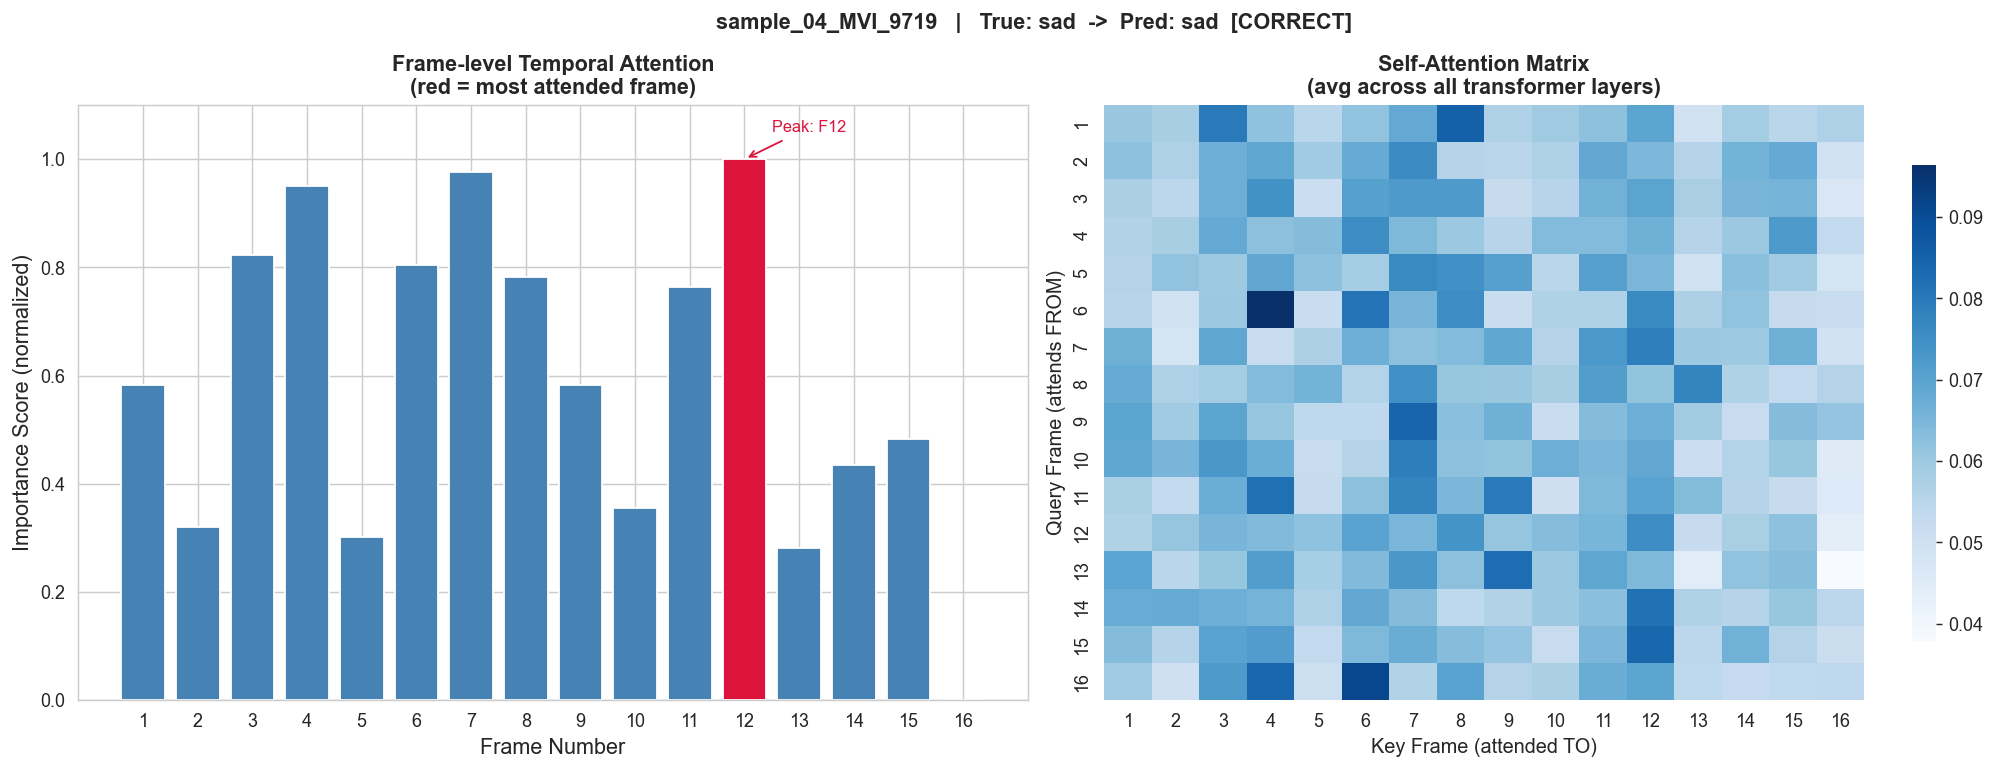
\includegraphics[width=\textwidth]{results/de5ad801-1a1d-4308-9073-05ff3b7f334f.png}
\caption{Temporal attention visualization for a correctly classified sad sample.}
\label{fig:attention_sad}
\end{figure*}

\begin{figure*}[t]
\centering
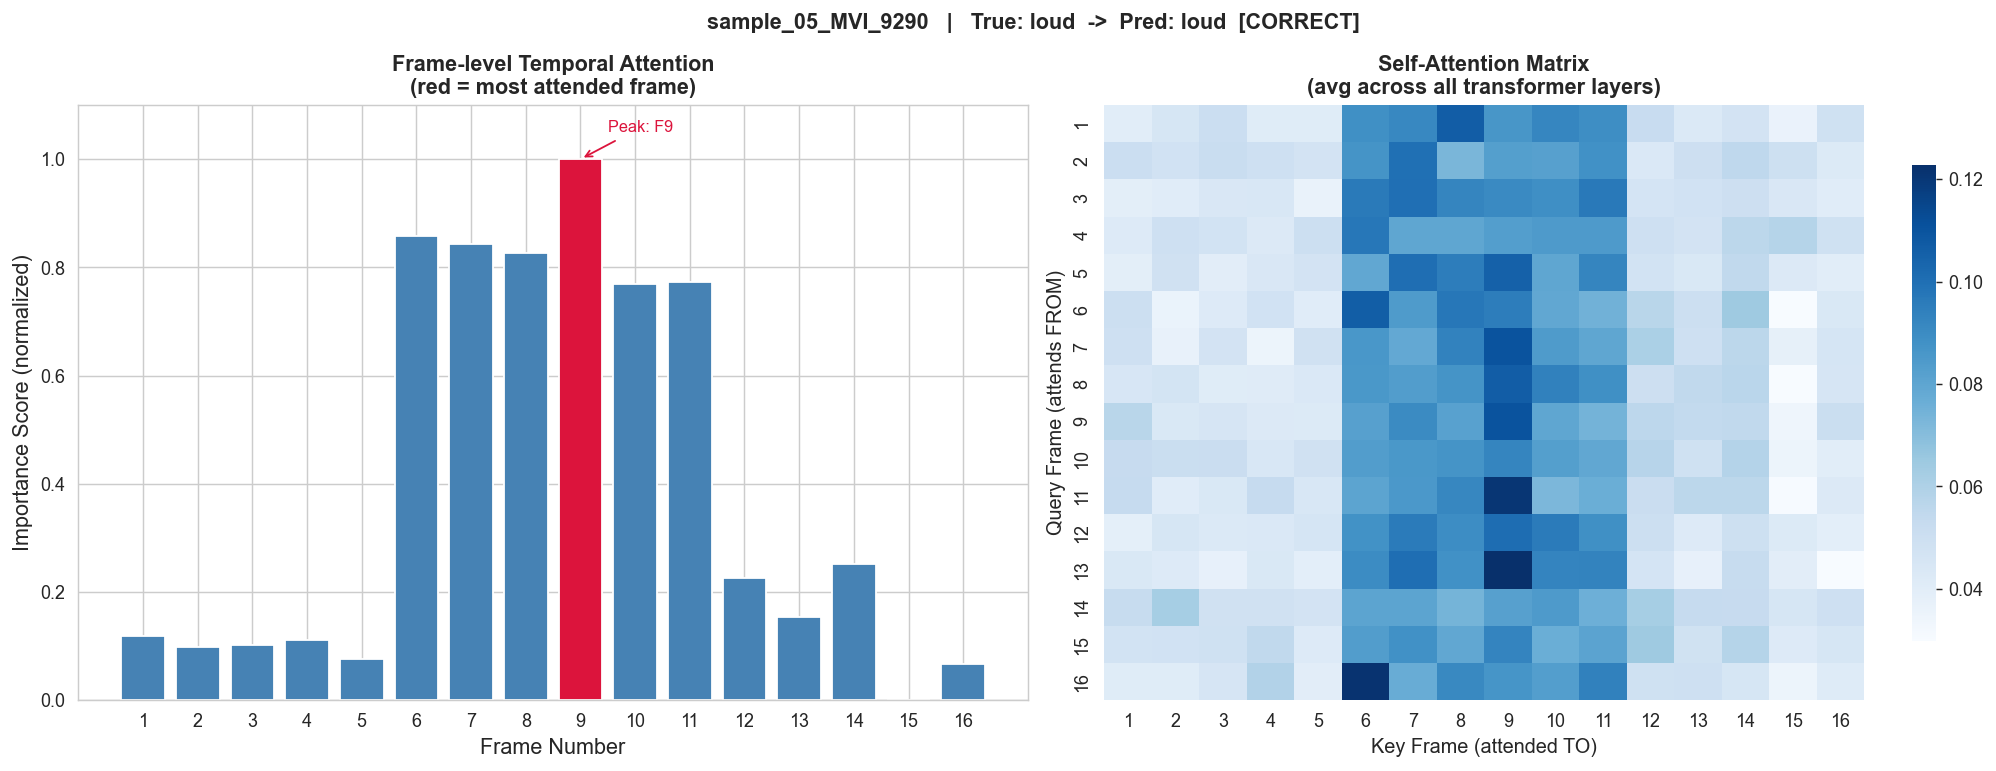
\includegraphics[width=\textwidth]{results/9382eda1-0a79-4bac-98af-59e3e8a9182a.png}
\caption{Temporal attention visualization for a correctly classified loud sample.}
\label{fig:attention_loud}
\end{figure*}

\section{Discussion}

The results demonstrate that RGB-based visual features are the strongest modality for the selected subset. Late fusion matches the RGB baseline and improves Macro F1-score, showing that pose information can support prediction when combined carefully. However, pose-only recognition is weak, indicating that landmark trajectories alone are not sufficient under the current experimental conditions.

Adaptive fusion provides interpretability by learning modality weights. Although it does not improve test accuracy in this experiment, it reveals that the model considers pose trajectories important. This finding is useful for future work because it shows that better pose preprocessing and larger datasets may improve adaptive multimodal learning.

\section{Conclusion and Future Work}

This paper presented an Adaptive Multi-Modal Fusion Transformer for Indian Sign Language recognition. The proposed system combines RGB video frames and pose landmarks using Transformer-based temporal modelling. Five configurations were evaluated on an eight-class INCLUDE subset. RGB baseline and late fusion achieved the highest test accuracy of 81.82\%, while adaptive fusion learned interpretable modality weights with 85.2\% importance assigned to pose.

Explainability analysis using Grad-CAM and temporal attention maps confirmed that the model focuses on hand-arm regions and middle gesture frames. Future work will focus on training with the full INCLUDE dataset, increasing the number of sign classes, improving pose landmark preprocessing, applying modality dropout, and exploring cross-attention fusion mechanisms.

\begin{thebibliography}{00}

\bibitem{resnet}
K. He, X. Zhang, S. Ren, and J. Sun, ``Deep Residual Learning for Image Recognition,'' in \textit{Proc. IEEE Conference on Computer Vision and Pattern Recognition}, 2016.

\bibitem{transformer}
A. Vaswani et al., ``Attention Is All You Need,'' in \textit{Advances in Neural Information Processing Systems}, 2017.

\bibitem{mediapipe}
C. Lugaresi et al., ``MediaPipe: A Framework for Building Perception Pipelines,'' arXiv preprint arXiv:1906.08172, 2019.

\bibitem{gradcam}
R. R. Selvaraju et al., ``Grad-CAM: Visual Explanations from Deep Networks via Gradient-based Localization,'' in \textit{Proc. IEEE International Conference on Computer Vision}, 2017.

\bibitem{gcn}
S. Yan, Y. Xiong, and D. Lin, ``Spatial Temporal Graph Convolutional Networks for Skeleton-Based Action Recognition,'' in \textit{Proc. AAAI Conference on Artificial Intelligence}, 2018.

\bibitem{multimodal}
A. Zadeh et al., ``Tensor Fusion Network for Multimodal Sentiment Analysis,'' arXiv preprint arXiv:1707.07250, 2017.

\bibitem{survey}
T. Baltrusaitis, C. Ahuja, and L.-P. Morency, ``Multimodal Machine Learning: A Survey and Taxonomy,'' \textit{IEEE Transactions on Pattern Analysis and Machine Intelligence}, 2019.

\bibitem{isl}
P. V. V. Kishore and P. R. Kumar, ``Segmenting Hands and Face in Indian Sign Language Gestures,'' \textit{International Journal of Computer Applications}, vol. 47, no. 5, pp. 12--20, 2012.

\end{thebibliography}

\end{document}